\documentclass{article}
\usepackage{graphicx}
\usepackage{float}
\usepackage{hyperref}
\begin{document}

\title{Exoplanet Search: Vetting Kepler Light Curves}
\author{Praveen Gowtham}
\date{}
\maketitle
\section{Introduction/Background}
\paragraph{}
In 1992 astronomers discovered a periodic set of dips modulating the emission from a pulsating neutron star. The source of these dips was identified as two planetary bodies orbiting the neutron star. The possibility of discovering and examining planets that do not orbit our sun was a compelling one. Some relevant reasons include the desire to find Earth-similar planets that could host extra-terrestrial life, or to understand the distribution of the types of planets and planetary systems that exist and where our own solar system fits in this schema.

 A swarm of activity in exoplanet detection technique development and the creation of theoretical frameworks for extracting information about these planets soon emerged. This project focuses on one of these techniques: light curve transit detection. In this technique, the light flux of a target star is observed for an extended period of time (months to years) by a telescope. An orbiting planet can transit across the line of sight between the star and the telescope which results in a small dip in the measured light intensity of the star. \textit{Note: these dips are usually quite small compared to the overall stellar light intensity.} An illustration of a planetary transit and its effects on a stellar light curve can be seen below:
 
 \begin{figure}[H]
 	\begin{center}
 		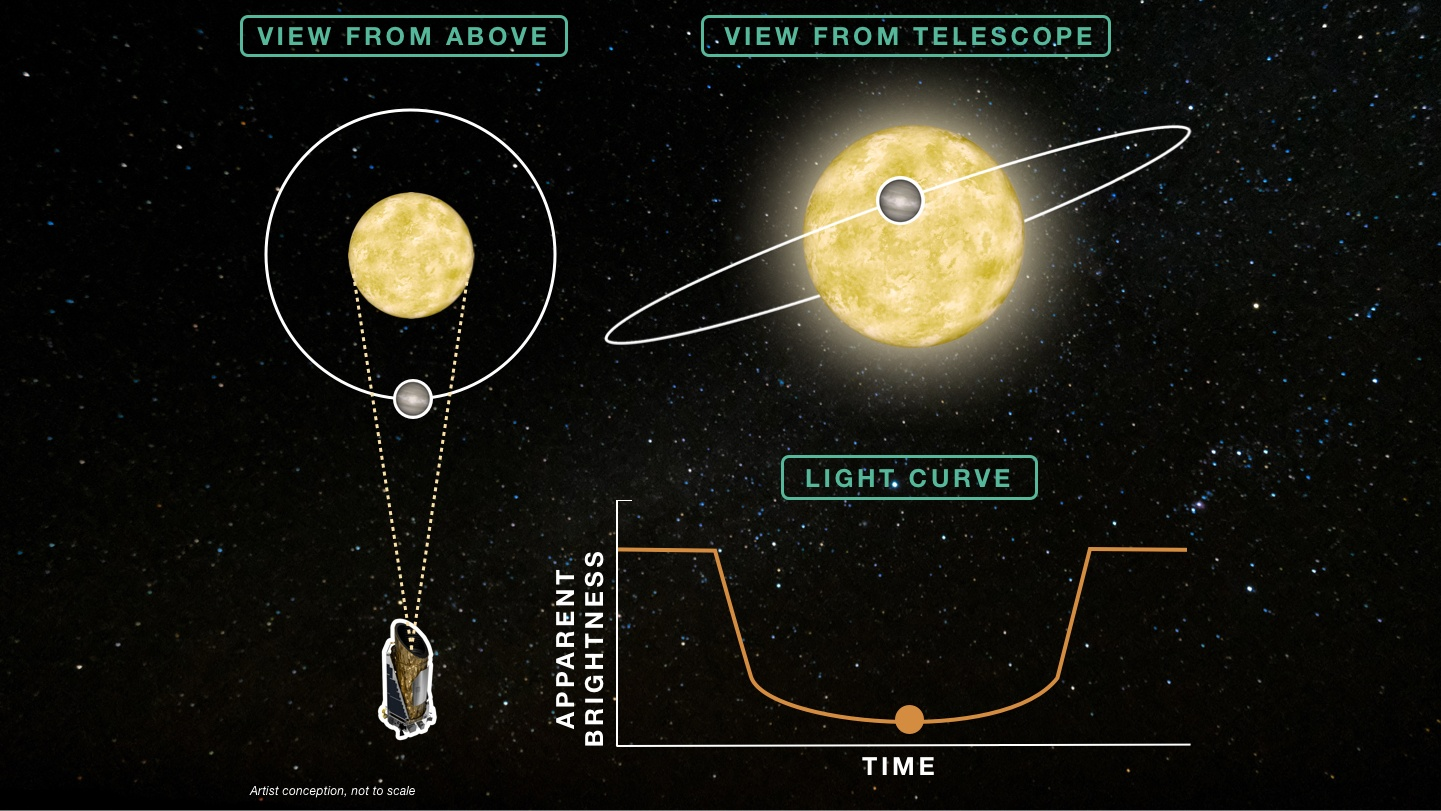
\includegraphics[totalheight=5cm]{figures/transit_illustration.jpg}
 	\end{center}
 \caption{Exoplanet transit.}
 \end{figure}

\paragraph{}
These dips will occur at regular intervals corresponding to the orbital period of the planet about the host star. Here is an example showing a real light curve with periodic dips in the light curve:
 \begin{figure}[H]
	\begin{center}
		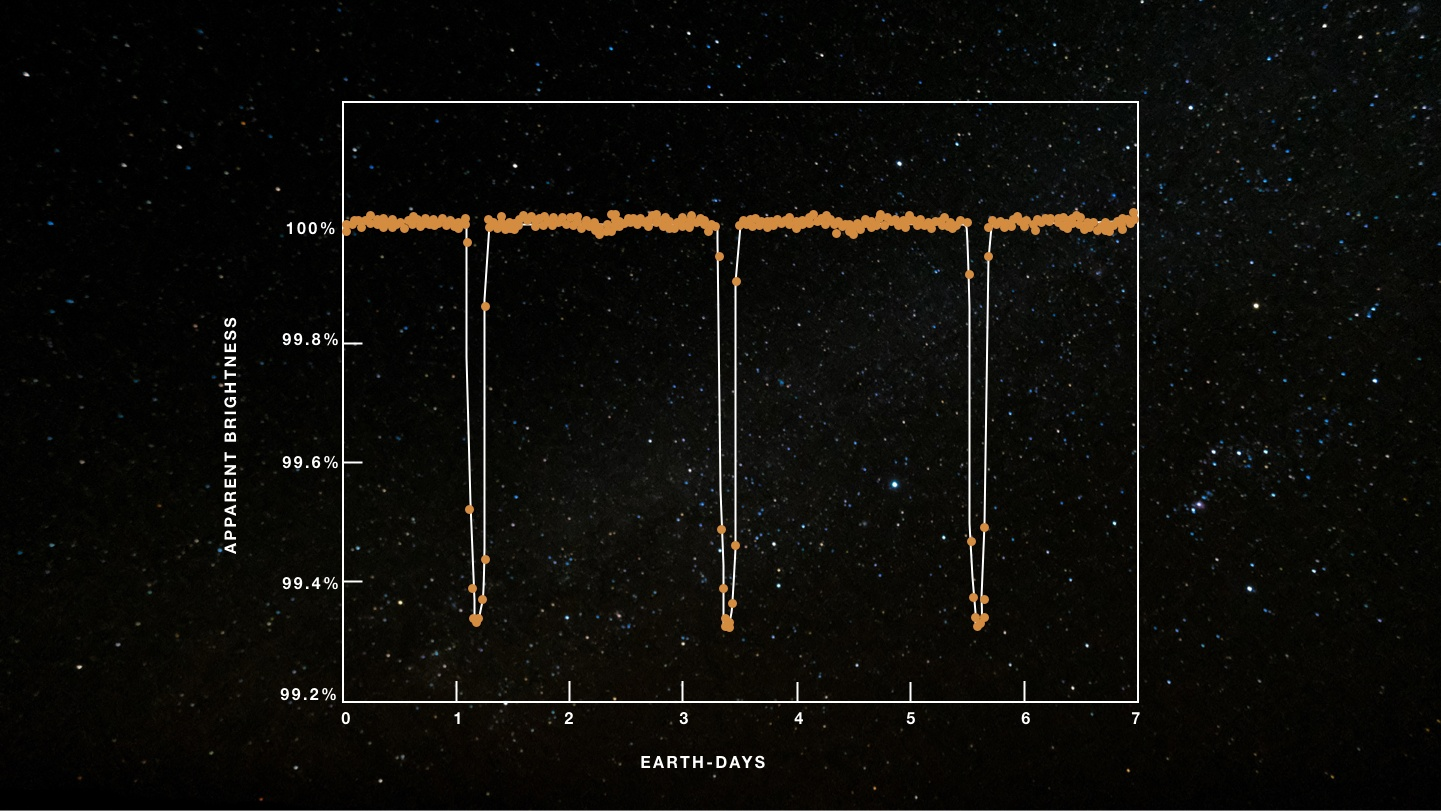
\includegraphics[totalheight=6cm]{figures/exo_multiple_transit.jpg}
	\end{center}
	\caption{Multiple transits from exoplanet HAT-P-7 b.}
\end{figure}
\paragraph{} The shape, the depth, and the period of these transits along with stellar parameters yields a wealth of information about the exoplanet: it's radius, mass, surface temperature, orbital parameters around the star, etc. 
So far, over 3000 exoplanets and their properties have been discovered using the light curve transit detection method. 
\paragraph{} So what's the problem? The example from HAT-P-7 b has an exceptionally clear planetary transit signal. More often than not, the transits are significantly shallower. In such cases a decision must be made on whether a dip in the light curve is actually a planetary transit or stellar noise. Stellar noise can be quite significant. The surface of stars are full of eruptions, temporary local cool spots (sunspots), plasma turbulence, not to mention the inevitable fluctuations coming from the fact that a star is hot. 
In addition, there are non-planetary phenomena that can produce statistically significant periodic dips. Among these are orbiting binary star systems or variable stars that pulsate or produce light intensity chirps. There are also imaging artifacts that come from the light of another star periodically leaking into the measured intensity of a target star. Light curves from binary star systems, in particular, can closely mimic that of an exoplanetary transit about a host star. The two stars orbit about each other and both partially eclipse the other at different phases of the orbital cycle. Since both stars produce a significant amount of light we will expect two eclipses. The primary eclipse (deepest dip in the light curve) occurs when the less luminous star comes in front of the more luminous star. The secondary eclipse occurs when the reverse is true. The relative depths of the two eclipses will depend on the magnitude/size of the two stars in relation to each other. An example can be seen below:
 \begin{figure}[H]
	\begin{center}
		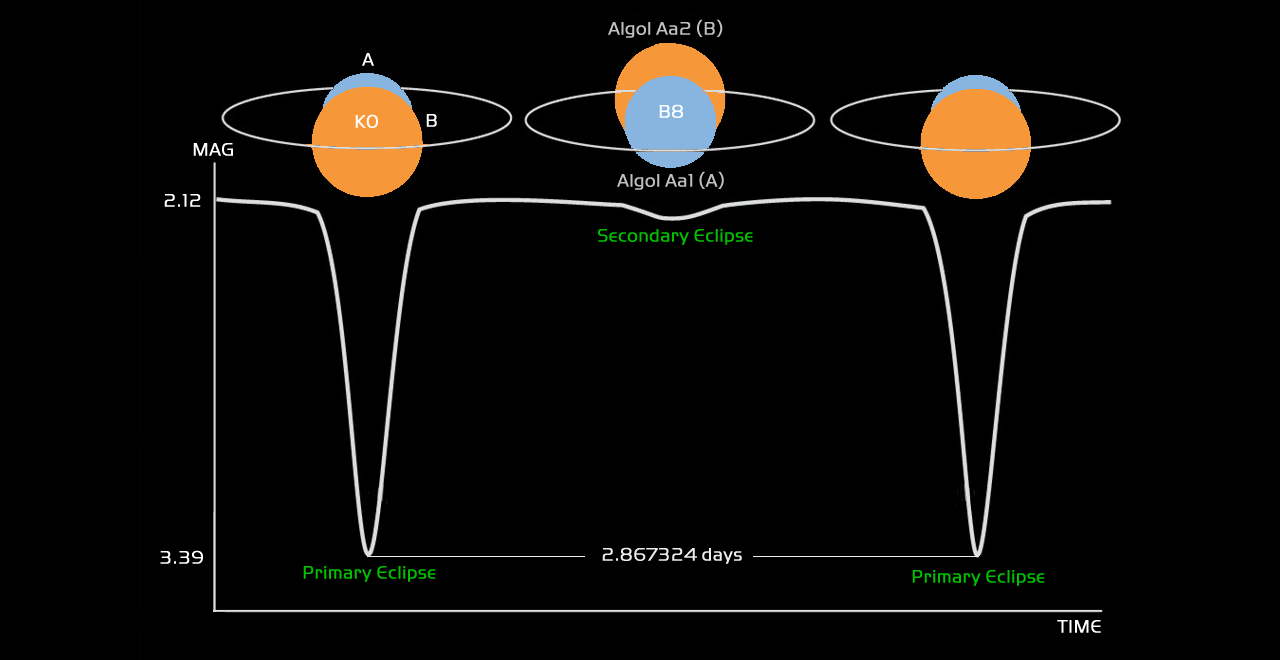
\includegraphics[totalheight=6cm]{figures/algol-curve.png}
	\end{center}
	\caption{Light curve from the Algol A/B binary star system.}
\end{figure}

\paragraph{} These look a lot like the curves for exoplanets. But as can be seen, there are differences -- such as the existence of a secondary eclipse. Planets only reflect light from their host star. Thus, with the exception of some very large planets with small orbital radii (known as hot Jupiters) real exoplanet secondary eclipses are undetectable. Even in the case of hot Jupiters, secondary eclipses typically have much smaller amplitude dips in the light curves than the secondary eclipses associated with a binary star companion. There are other more subtle difference in the light curves of binary star systems vs exoplanets which will be discussed later. But it is clear that making a decision on whether a star has an exoplanet via transit detection will first involve the determination of statistically significant periodic transit-like events  \textit{and} the vetting of potential false positives (binary stars or other phenomena) in the remaining light curves. \textbf{This project aims to construct relevant features from light curves with statistically significant events and make determinations as to whether the event and light curve correspond to an exoplanet, a binary star system, or some other phenomena.} 
\section{Data Wrangling}
\subsection{Data Sources}
\paragraph{}All the data in this study come from the Kepler Space Telescope. The telescope was launched into Earth orbit in 2009 and decommissioned in 2018. Kepler was tasked with long term observation of a section of our Milky Way galaxy and in the end managed to observe approximately 500,000 stars. Of these stars, only a small fraction had light curves that contained statistically significant events that could potentially be transits. 
 \begin{figure}[H]
	\begin{center}
		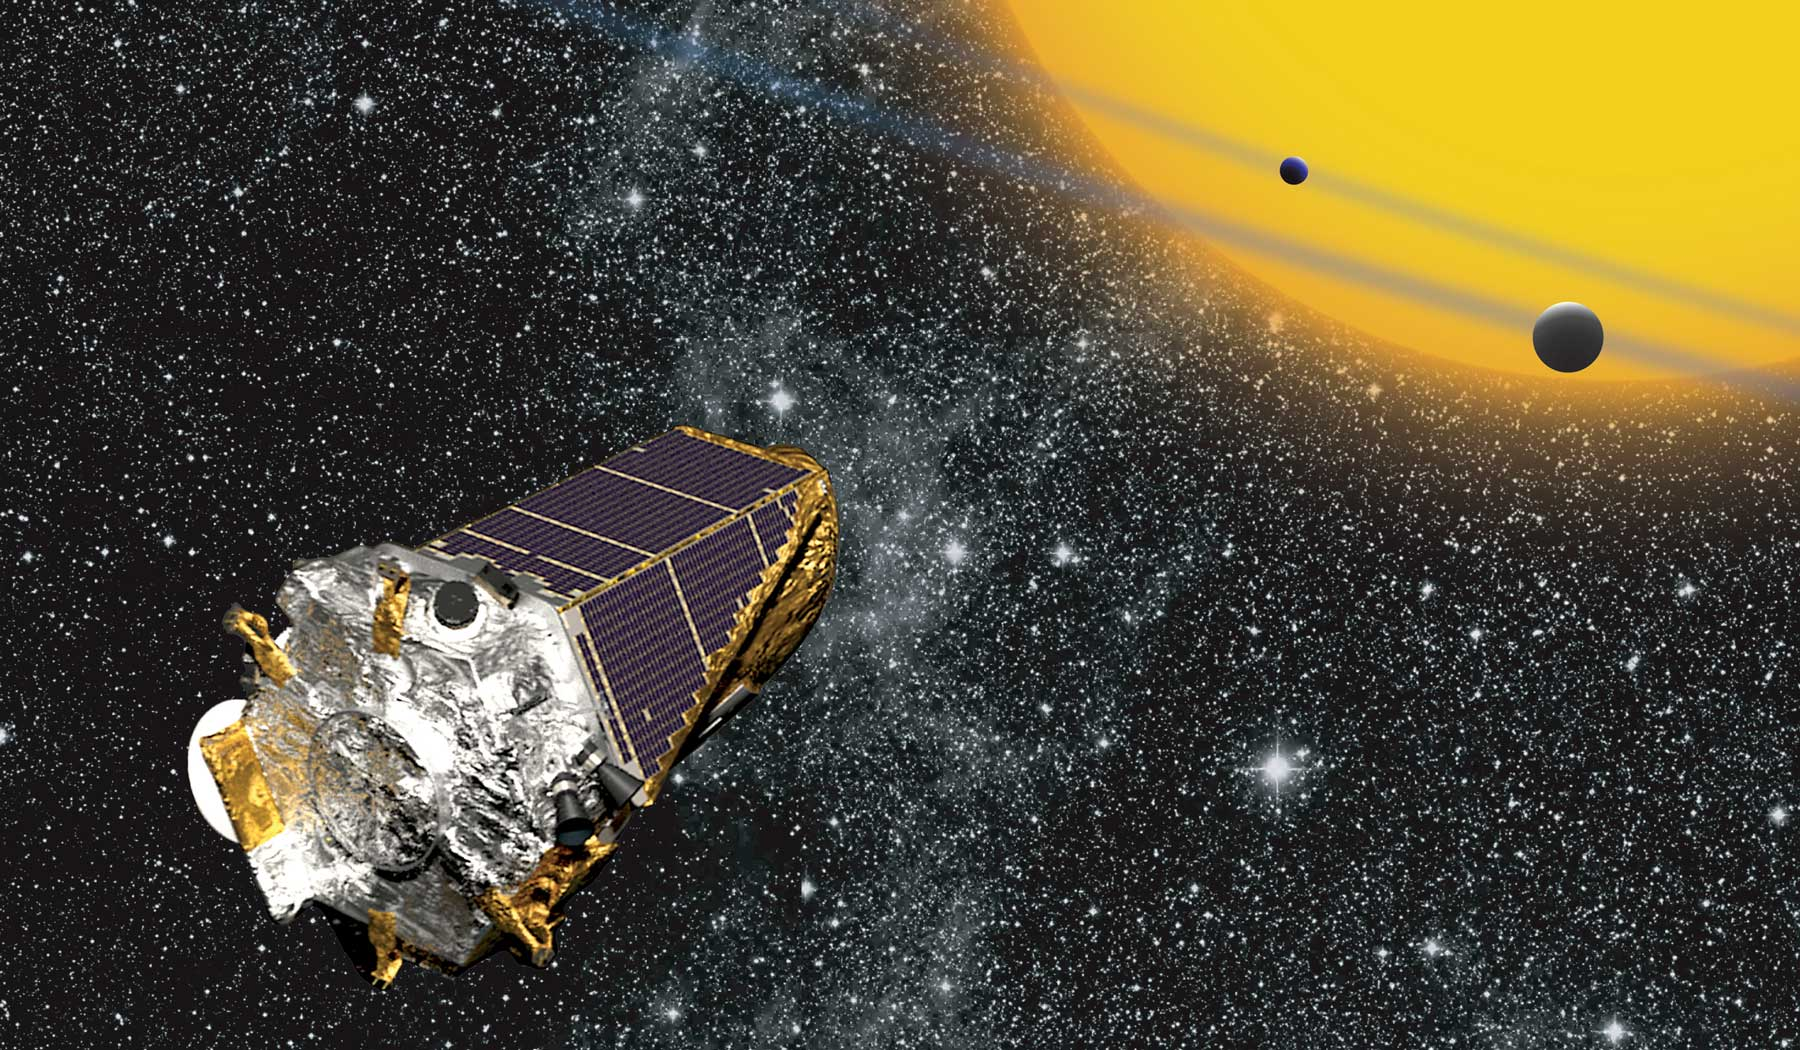
\includegraphics[totalheight=6cm]{figures/kepler_spacetelescope.jpg}
	\end{center}
	\caption{Kepler Space Telescope}
\end{figure}
\paragraph{} The Kepler mission developed a data pipeline in order to store the surveyed stellar light curves, flagging potential objects of interest with statistically significant events (known as Kepler Objects of Interest or KOIs), and generating transit parameters like the period, depth, and duration of the transits. These KOIs are the target stars that we are interested in developing a model for with the the hope that the model can vet between true exoplanets and false positives. The light curves and the aggregated data for the Kepler mission KOIs are stored in the Minkulski Archive for Space Telescopes (MAST) and the NASA Exoplanet Archive. \\

Light curve request API: \\ \href{https://exo.mast.stsci.edu/docs/getting_started.html}{https://exo.mast.stsci.edu/docs}

Aggregated/cumulative data table: \\ \href{https://exoplanetarchive.ipac.caltech.edu/docs/program_interfaces.html}{https://exoplanetarchive.ipac.caltech.edu/docs/program\textunderscore interfaces.html}

\paragraph{}
The cumulative data table contains transit parameters/metadata about the KOIs. The KOIs are indexed by the Kepler input catalog star ID (KIC ID) and transit event number. The transit event number (TCE num) is relevant when there is more than one planet orbiting the target star with a particular KIC ID. Each number would correspond to a different planet in the system. The cumulative table contains info like the period, maximum depth, and duration of the transit event. There are also flags for the status of a given KOI (confirmed planet, secondary eclipse false positive, non-transiting phenomenon, etc.). \textbf{We used the flags in the cumulative table as training labels. Our aim is to separate the light curves into three classes: exoplanets, secondary eclipse FPs, and non-transit phenomena (NTP) FPs.}  

\begin{table}[H]
	

\begin{tabular}{|c|c|c|c|}
	\hline
	Class name & Confirmed Planet  & Secondary Eclipse FP   &  NTP FP  \\
	\hline
	Target Label & 1  & 2 & 3    \\
	\hline

\end{tabular}
\caption{Class name and label encoding scheme.}
\end{table}

\paragraph{} 
The KIC ID and TCE num of a transit crossing event (TCE) in the cumulative table can be used to specify a light curve request for the given transit from the MAST API. The indices are requisite parameters passed to the constructor for a custom class KOIObject within the module KOIclass. The class performs a whole host of functions and sweeps many of the details of data downloading, light curve signal processing, feature construction, and light curve plotting under the rug. Raw light curve data was downloaded to disk as this allows construction of the light-curve extracted feature matrix and subsequent transformations/changes to this matrix to occur with much higher throughput. 

\section{Light Curve Processing}
The detrended light curves needed to go through a few preprocessing steps before feature extraction could commence. In short, the light curves were phase-folded (for a periodic signal, points at a certain phase in the oscillation are grouped together). These grouped points are averaged together to yield the phase-folded, bin-averaged light curve. This procedure helps in averaging out some of the Gaussian noise and keeps the cycle-averaged periodic signal. The primary transit crossing event is indexed to zero phase. The steps are shown below:

 \begin{figure}[H]
	\begin{center}
		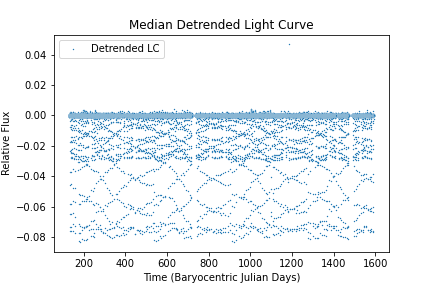
\includegraphics[totalheight=5cm]{figures/lc_detrend_secondaryFP_ex1.png}
	\end{center}
	\caption{Detrended light curve from Kepler data validation pipeline}
\end{figure}
The above light curve is clearly periodic. We phase-fold the light curve on this period, bin the data, and average.
 \begin{figure}[H]
	\begin{center}
		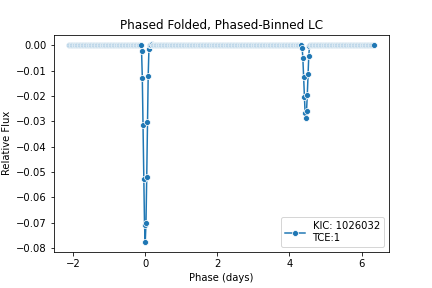
\includegraphics[totalheight=5cm]{figures/phasefolded_secondaryFP_ex1.png}
	\end{center}
	\caption{Phase-folded and average light curve. This is a binary star system.}
\end{figure}

\section{Feature Extraction}
We extract features from these phase-folded and averaged light curves. We want to construct features from these time-series that help our models to distinguish between the different classes. A look at representative curves for the three classes will be helpful. A representative phase-folded/averaged for class 2 (secondary eclipse FP) has already been seen in Fig 6. Examples for NTP FPs and confirmed planets can be seen below:
 \begin{figure}[H]
	\begin{center}
		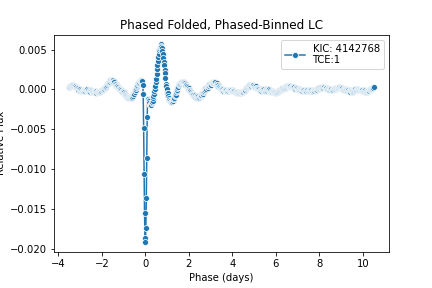
\includegraphics[totalheight=5cm]{figures/phasefolded_ntp_ex2.png}
	\end{center}
	\caption{Phase-folded and average light curve in the NTP FP class. Example of a pulsating star.}
\end{figure}
 \begin{figure}[H]
	\begin{center}
		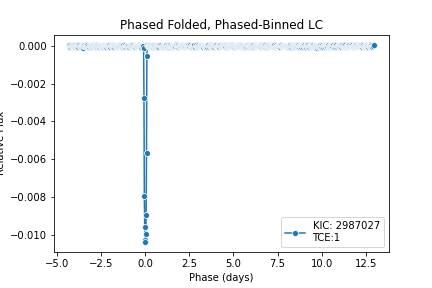
\includegraphics[totalheight=5cm]{figures/phasefolded_CP_ex1.png}
	\end{center}
	\caption{Phase-folded and average light curve for a confirmed exoplanet.}
\end{figure}

\paragraph{}These light curves suggest the construction of a few features that could help distinguish between the various classes. In order to differentiate class 2 (Fig 6) and class 1 (Fig 8), we need to conduct a statistical test on the existence of a secondary peak. This is done by subtracting the primary TCE and performing a statistical test for the existence of a secondary eclipse against the noise background. We call the resulting statistic the \textbf{weak secondary statistic} and is referred to for shorthand as $p_{sec}$. It measures the likelihood that a secondary peak is not noise.

\paragraph{} In a subset of the secondary eclipse FPs, the secondary eclipse occurs pretty close to half period. In cases where this secondary eclipse's amplitude is large enough, the Kepler pipeline's statistical tester logs this event as the same as the primary event. The effect is that the Kepler pipeline outputs a period that is actually half the period of the binary system. An example can be seen below:

 \begin{figure}[H]
	\begin{center}
		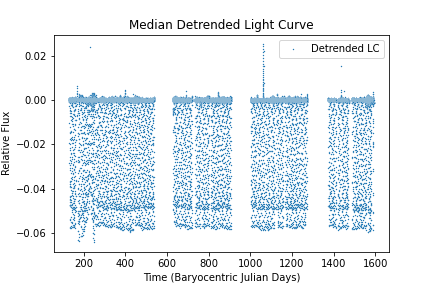
\includegraphics[totalheight=5cm]{figures/lc_detrend_secondaryFP_ex2.png}
	\end{center}
	\caption{Detrended light curve for secondary FP with large amplitude secondary eclipse.}
\end{figure}
A naive phase-folding/averaging according to the Kepler pipeline's extracted period would yield a single transit dip: thus superimposing the primary and secondary eclipse and averaging them. To account for this possibility, we group alternating cycles together into even or odd phase groups and average within the subgroups. We've staggered the even and odd phase averages by the Kepler pipeline period and plotted the result of this operation below:
  \begin{figure}[H]
 	\begin{center}
 		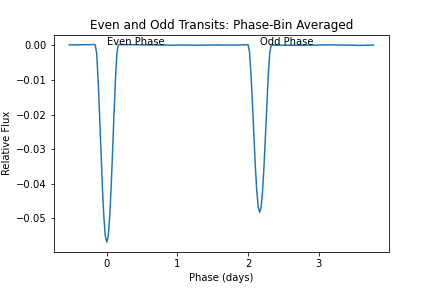
\includegraphics[totalheight=5cm]{figures/evenoddstagger_secondaryFP_ex2.png}
 	\end{center}
 	\caption{Period-staggered even and odd phase-folded/averaged series corresponding to light curve from Figure 9. The even and odd transit amplitudes clearly differ indicating that this is a secondary eclipse FP.}
 \end{figure}
\paragraph{} This all suggests a statistical test: collect transit depths for even and odd cycles. Then do a 2-sample t-test to determine if the difference of the means of the transit depths between the alternating cycles is statistically significant. The t-statistic itself can be used here as a feature. Larger t-statistics imply that we can reject the null (that the even/odd cycle amplitudes are the same) with higher certainty. We call this the \textbf{even-odd statistic} and observations with large even odd statistic are likely secondary eclipse false positives.
\paragraph{} Some generic statistical features are also of use here as well. The depth of the primary transits (or the minimum value of the phase-binned light curve) is also used as a feature. Secondary eclipse FPs from binary stars tend to have much larger transit depths than those from exoplanets -- as can bee seen by looking at Fig 6 and Fig 8. Non-transiting FPs have a lot of wiggles and can often have max values in the series that are large positive compared to base-line. Thus we also take the max as a feature.
\paragraph{}
We have spent a lot of time on statistical tests for secondary eclipse phenomena or generic statistical features of the light curve. But there is quite a lot of information in the shape of the TCEs themselves that can help us distinguish between the three classes. For each light curve, we zoom in on the primary transit event and extract the light curve localized at $\pm 2$ durations on either side of the zero phase of the transit. In order to make faithful comparisons of the shape of the transits across different observation and classes, we normalize the time axis (x-axis) by the transit duration and rescale the relative flux (y-axis) to lie between [0,-1] with -1 being the transit depth. The xy-rescaled transit close-ups are then resampled into fixed length series of 141 points. These 141 bins of the xy-normalized transit close-ups are incorporated into the feature matrix. Below, we can see the results of this process across the secondary eclipse FPs and confirmed planets:
 \begin{figure}[H]
	\begin{center}
		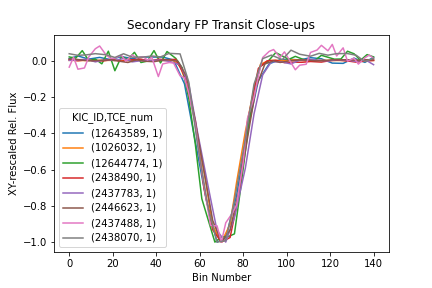
\includegraphics[totalheight=5cm]{figures/rescalexy_secondaryFP.png}
	\end{center}
	\caption{XY-rescaled transit close-ups for secondary eclipse FPs (class 2). }
\end{figure}
\begin{figure}[H]
	\begin{center}
		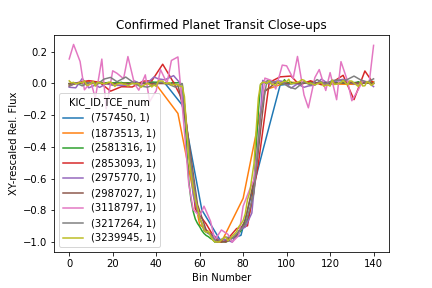
\includegraphics[totalheight=5cm]{figures/rescalexy_CP.png}
	\end{center}
	\caption{XY-rescaled transit close-ups for confirmed exoplanets(class 1).}
\end{figure}
The secondary eclipse FP transit close-ups all collapse to a V-like shape when rescaled. On the other hand, the confirmed planet class transit close-ups collapse to something approximatng a U-shape. We haven't plotted the curves for class 3 (non-transiting phenomena) as there is much higher variability in the series across observations (making for an unenlightening plot). The important point is that the shape of the transit encoded in the 141 bins clearly provide a means of distinguishing between the classes.
\paragraph{} Finally, the transit duration (measured in hours) and the TCE period from the Kepler cumulative table are included in the feature matrix. The following table summarizes the features extracted from the light curves:

\begin{table}[H]
	\begin{tabular}{|c|c|}
		\hline
		Period &  TCE period (days) from Kepler cumulative table,\\
		\hline
		Duration & TCE duration (hours) from Kepler cumulative table. \\
		\hline
		even\_odd\_stat & Even-odd statistic for secondary eclipse detection. \\
		\hline
		p\_secondary & Weak secondary statistic  \\
		\hline
		min & Almost always corresponds to the depth of the primary transit.  \\
		\hline
		max & Maximum value in phase-folded/bin-averaged light curve. \\
		\hline
		LCBIN\_0 - LCBIN\_140 & 141 points of the xy-normalized primary transit close-ups  \\
		\hline
	\end{tabular}
\caption{Features extracted from Kepler data pipeline.}
\end{table}
\section{Statistical EDA on some features}
We spent some time constructing features. Are these features useful? We'll answer the question for some of these in this report. Analysis on all of the features can be found in the notebooks. For what proceeds in this report, all the features have been normalized already. We look at the weak secondary statistic:

  \begin{figure}[H]
	\begin{center}
		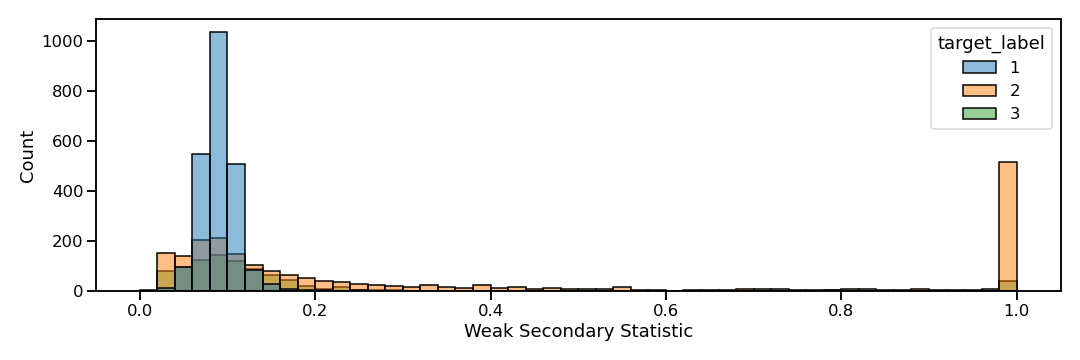
\includegraphics[totalheight=4cm]{figures/psec_hist.png}
	\end{center}
	\caption{Distribution of weak secondary statistic. As designed, higher values indicate a secondary eclipse FP. Large number of counts at 1.0 has to do with the way we constructed the feature. }
\end{figure}
  \begin{figure}[H]
	\begin{center}
		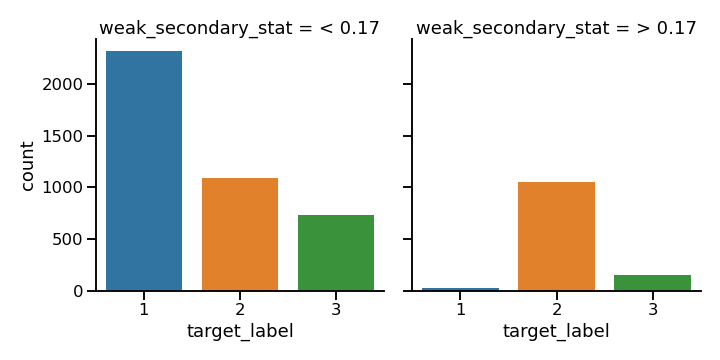
\includegraphics[totalheight=4cm]{figures/psec_class_diff.png}
	\end{center}
	\caption{Bar plot showing that the weak secondary statistic preferentially selects out class 2 at larger values. }
\end{figure}
The even-odd statistic shows similar selection for class 2 at higher values. Both statistics are doing what they should be doing and will be good features for our models to train on.
  \begin{figure}[H]
	\begin{center}
		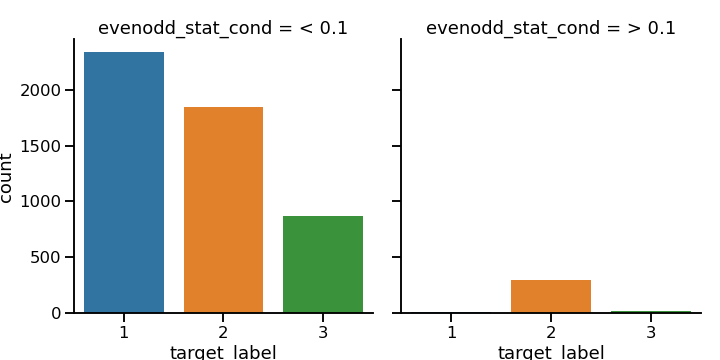
\includegraphics[totalheight=4cm]{figures/evenodd_class_diff.png}
	\end{center}
	\caption{Bar plot showing that the even-odd statistic preferentially selects out class 2 at larger values. }
\end{figure}
One of the features that aids in selecting out NTPs over the other two classes is the period. We've plotted the cumulative distribution function of the three classes with respect to the TCE period: 
  \begin{figure}[H]
	\begin{center}
		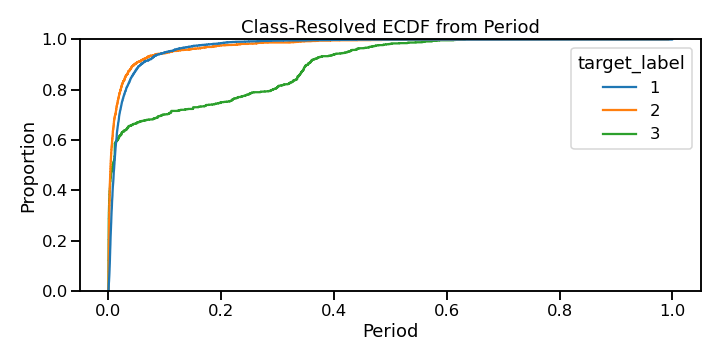
\includegraphics[totalheight=4cm]{figures/ecdf_period.png}
	\end{center}
	\caption{Empirical cumulative distribution of the TCE period conditioned on the three classes. }
\end{figure}
Class 3 has a long tail and dominates the long period sector of the TCEs. The period will thus be a good feature to select for the NTPs. The other features min, max, and duration are also useful in one way or another for selecting or differentiating between classes. The LCBIN features will be discussed in the next section.
\section{Last Pre-processing: Dimensionality Reduction on Transit Close-Up Features}
\paragraph{} The 141 transit close-up features are useful but form a feature sub-space of high dimensionality. This typically presents some problems for machine learning algorithms. But as we can see from Figures 11 and 12 the true dimensionality of the space that the close-up features live on is much lower. We employ a dimensionality reduction technique called Locality Preserving Projections (LPP). As the name suggests, this technique projects from high dimensions to a low dimensional space in a way that preserves neighborhoods. Details can be found in He and Nyogi (NIPS, 2003). XY-rescaled transit close-ups with U-shapes corresponding to exoplanets should be closer to each other than to those from eclipsing binary stars and NTPs in the low-D space generated by LPP. We perform LPP on the light curves with knn segmentation at 5 and a target dimension of 2. We plot the resulting distributions for three classes in this 2D space:

  \begin{figure}[H]
	\begin{center}
		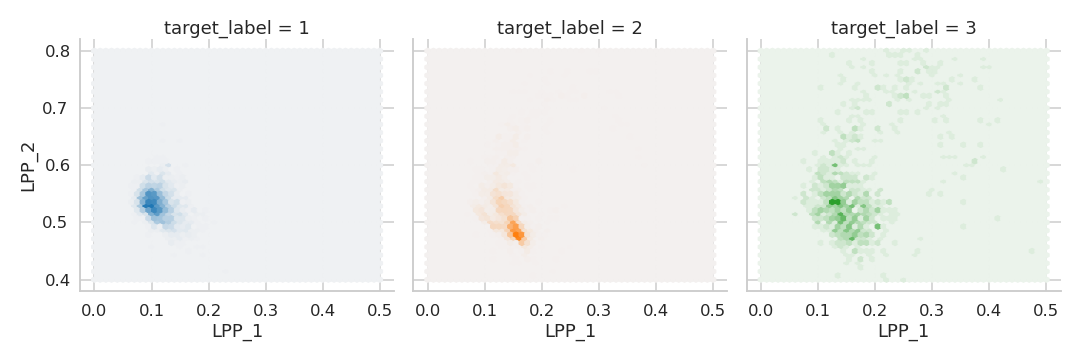
\includegraphics[totalheight=4cm]{figures/lpp_hexbinplot.png}
	\end{center}
	\caption{Distribution for each class in the 2D space generated by LPP. Target label 1, 2, and 3 correspond to confirmed planet, secondary eclipse false positives, and non-transiting phenomena respectively.}
\end{figure}
While there is certainly overlap between the classes, class 1 and 2 have the bulk of their distribution centered at different areas in the 2D-space. Class 3 has a bit more overlap with class 2. The reason for the overlap has to do with the fact that some Class 3 light curves look like eclipsing binaries and that additional information not present in the light curve is required to differentiate them from class 2. However, class 3 does dominate extremal parts of the 2D space. Our conclusion then is that the projected 2D feature set  (LPP\_1, LPP\_2) is a good one and will help the models in differentiating between classes. The final feature set that we fed into the models is: 
\begin{table}[H]
	\begin{tabular}{|c|c|}
		\hline
		Period &  TCE period (days) from Kepler cumulative table,\\
		\hline
		Duration & TCE duration (hours) from Kepler cumulative table. \\
		\hline
		even\_odd\_stat & Even-odd statistic for secondary eclipse detection. \\
		\hline
		p\_secondary & Weak secondary statistic  \\
		\hline
		min & Almost always corresponds to the depth of the primary transit.  \\
		\hline
		max & Maximum value in phase-folded/bin-averaged light curve. \\
		\hline
		LPP\_1 & First dimension of LPP-reduced XY-rescaled transit close-ups  \\
		\hline
		LPP\_2 & Second dimension of LPP-reduced XY-rescaled transit close-ups . \\
		\hline
	\end{tabular}
	\caption{Final feature set used for model training}
\end{table}
\section{Modeling}
\paragraph{} We split the data into 85-15 training/hold-out set. Within the training set, we then conducted 5-fold cross validation for each model trained with a 85-15  training/evaluation split. We tried three classifier types: a random forest classifier, an RBF-kernelized soft-margin SVM, and a gradient boosting classifier. The models were incorporated as the last step in a pipeline that did all the necessary fit/transformations (e.g., LPP dim reduction, normalization, etc.) before fitting the classifier. We initiated a CV hyperparameter search on the pipelines to tune model performance for each class. The pipeline architecture shines here as it ensures prevention of data leakage during cross validation and in the final model transformation/fitting stages. We chose to optimize our CV on the F1 score micro-averaged across classes. The best performing models (within the hyperparameters scanned) as deemed by the CV scores are listed below: \\
\textbf{Random Forest}:\\ RandomForestClassifier(max\_depth=18, max\_features=3, n\_estimators=700) \\ 
\textbf{RBF-Kernelized Soft-Margin SVM}: \\ SVC(C=100, gamma=25) \\
\textbf{XGBoost}:\\ XGBClassifier(learning\_rate=0.1, max\_depth=2, n\_estimators=1000) \\

\subsection{Random Forest Classifier: Results}
\begin{table}[H]
	\begin{center}
\begin{tabular}{l|r|r|r|r}
	
	{} &  precision &    recall &  f1-score &     support \\ \hline
	
	1            &   0.925620 &  0.957265 &  0.941176 &  351.000000 \\ \hline
	2            &   0.858859 &  0.890966 &  0.874618 &  321.000000 \\ \hline
	3            &   0.787037 &  0.643939 &  0.708333 &  132.000000 \\ \hline
	accuracy     &   0.879353 &  0.879353 &  0.879353 &    0.879353 \\ \hline
	macro avg    &   0.857172 &  0.830723 &  0.841376 &  804.000000 \\ \hline
	weighted avg &   0.876213 &  0.879353 &  0.876375 &  804.000000 \\ \hline
	
\end{tabular}
	\end{center}
	\caption{Classification report for Random Forest on hold-out set. Class 1 = Exoplanets, 2 = Secondary Eclipse FPs, 3 = NTP FPs}
\end{table}
  \begin{figure}[H]
	\begin{center}
		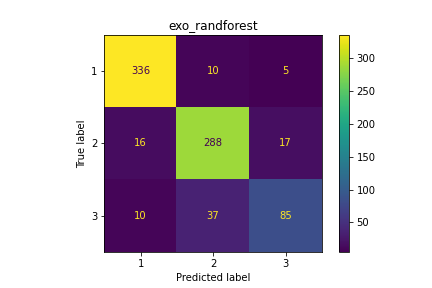
\includegraphics[totalheight=6cm]{figures/exo_randforest_cfmat.png}
	\end{center}
	\caption{Confusion matrix for the random forest on the hold-out set.}
\end{figure}
  \begin{figure}[H]
	\begin{center}
		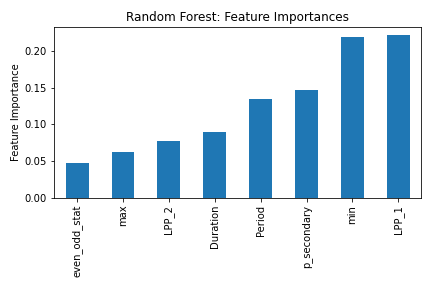
\includegraphics[totalheight=6cm]{figures/randforest_feature_imp.png}
	\end{center}
	\caption{Feature importances for Random Forest Model}
\end{figure}
\subsection{Kernelized SVM: Results}

\begin{table}[H]
	\begin{center}
\begin{tabular}{l|r|r|r|r}

	{} &  precision &    recall &  f1-score &     support \\ \hline

	Class 1            &   0.889764 &  0.965812 &  0.926230 &  351.000000 \\ \hline
	Class 2            &   0.854890 &  0.844237 &  0.849530 &  321.000000 \\ \hline
	Class 3            &   0.764151 &  0.613636 &  0.680672 &  132.000000 \\ \hline
	accuracy     &   0.859453 &  0.859453 &  0.859453 &    0.859453 \\ \hline
	macro avg    &   0.836268 &  0.807895 &  0.818811 &  804.000000 \\ \hline
	weighted avg &   0.855217 &  0.859453 &  0.855291 &  804.000000 \\ \hline

\end{tabular}
\end{center}
\caption{Classification report for SVM on hold-out set. Class 1 = Exoplanets, 2 = Secondary Eclipse FPs, 3 = NTP FPs}
\end{table}

\begin{figure}[H]
	\begin{center}
		\includegraphics[totalheight=6cm]{figures/exo_svc_cfmat.png}
	\end{center}
	\caption{Confusion matrix for the SVM on the hold-out set.}
\end{figure}
\subsection{XGBoost: Results}

\begin{table}[H]
	\begin{center}
\begin{tabular}{l|r|r|r|r}
	
	{} &  precision &    recall &  f1-score &    support \\ \hline
	
	1            &   0.943820 &  0.957265 &  0.950495 &  351.00000 \\ \hline
	2            &   0.867868 &  0.900312 &  0.883792 &  321.00000 \\ \hline
	3            &   0.773913 &  0.674242 &  0.720648 &  132.00000 \\ \hline
	accuracy     &   0.888060 &  0.888060 &  0.888060 &    0.88806 \\ \hline
	macro avg    &   0.861867 &  0.843940 &  0.851645 &  804.00000 \\ \hline
	weighted avg &   0.885601 &  0.888060 &  0.886128 &  804.00000 \\ \hline
	
\end{tabular}
	\end{center}
	\caption{Classification report for XGBoost on hold-out set. Class 1 = Exoplanets, 2 = Secondary Eclipse FPs, 3 = NTP FPs}
\end{table}
\begin{figure}[H]
	\begin{center}
		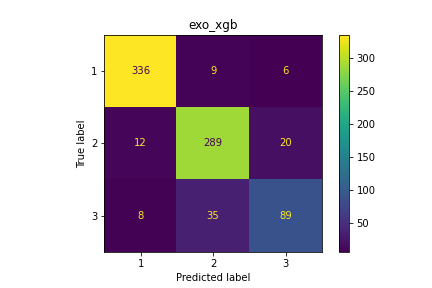
\includegraphics[totalheight=6cm]{figures/exo_xgb_cfmat.png}
	\end{center}
	\caption{Confusion matrix for the gradient boosting classifier on the hold-out set.}
\end{figure}
\begin{figure}[H]
	\begin{center}
		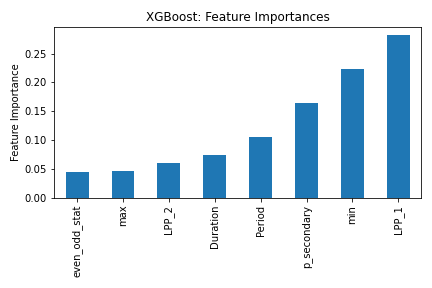
\includegraphics[totalheight=6cm]{figures/xgb_feature_imp.png}
	\end{center}
	\caption{Feature importances for XGBoost Model}
\end{figure}

\subsection{Modeling: Discussion}
\paragraph{} Model performance on the hold-out sets and in cross-validation (see notebooks for cross-validation performance) are comparable between the models. However, its clear that the tree ensemble models are outperforming the kernelized SVM. There are some general trends that all these models share. The first is that the precision/recall and F1 score on prediction in Class 1 are very good. \textbf{This implies that we are separating true exoplanets from false positives very well.} The models also do a solid job identifying secondary eclipse FPs. The predictions for class 3 are not amazing. The precision for class 3 across the models is fair, but the recall is not that great. This means that the model is identifying a significant number of light curves that are labeled as class 3 as some other class. A little digging shows that the models are marking these light curves as class 2 -- which is something we expected based on our EDA. But this is no worry, as in the end, we care about whether a light curve corresponds to an exoplanet or not.
\paragraph{}
In terms of the metrics and model complexity, XGBoost seems to be doing the best. The model has a similar number of trees as our optimal random forest but just with using stumps as opposed to trees with 18 layers. For class 1, the precision is 0.94, and the recall and f1-score is 0.95. For class 2, the precision is 0.87, and the recall is 0.90 and f1-score is 0.88. Not too shabby. I'd choose this model as the winner.
\paragraph{} The fact that these models are all performing well to varying degrees lends credence to the argument that the features we constructed and the feature engineering are key here. A look at the feature importances for the random forest and XGBoost corroborate this. All the features seem to be important with LPP\_1, min, and the weak secondary statistic being the most important. In fact, the feature importances are ranked exactly the same way for both models. This consistency is also a hint that the constructed features are a large part of what is driving the performance.
\section{Conclusions}
\paragraph{} It seems that we have built a pretty good light curve vetter for exoplanet transit identification within the Kepler Object of Interest catalog. Ongoing missions like Kepler 2 and TESS (Transiting Exoplanet Survey Satellite) are finding new objects of interest. They too have data validation pipelines that are pretty similar in architecture to the Kepler data validation stream. It would not take much to generalize our feature extraction, pre-processing and prediction pipeline appropriately and use it for light curve classification in other missions. 
\paragraph{} Ideally, we would have built a vetter that relies less on the mission data validation streams. We would need to incorporate instrument denoising, primary transit event detection, period extraction, and light curve whitening, and detrending on totally raw data. This is definitely a direction to go in that would actually cover the whole process end-to-end. But for now, our project does well for flagged objects of interest (which is what we intended to look at). The rest is for the future.

\end{document}

